\documentclass[tikz,border=7pt]{standalone}
\usepackage[scaled=0.95]{helvet}
\renewcommand{\familydefault}{\sfdefault}
\usetikzlibrary{arrows.meta,positioning,calc}
\definecolor{TEJNavy}{HTML}{1E2B55}
\definecolor{TEJBlue}{HTML}{1769AA}
\tikzset{
  block/.style={draw=TEJNavy,line width=1pt,minimum width=2.5cm,minimum height=1.1cm,align=center},
  sum/.style={draw=TEJNavy,circle,line width=1pt,minimum size=0.75cm},
  flow/.style={-{Latex[length=3mm]},TEJNavy,line width=1.2pt}
}
\begin{document}
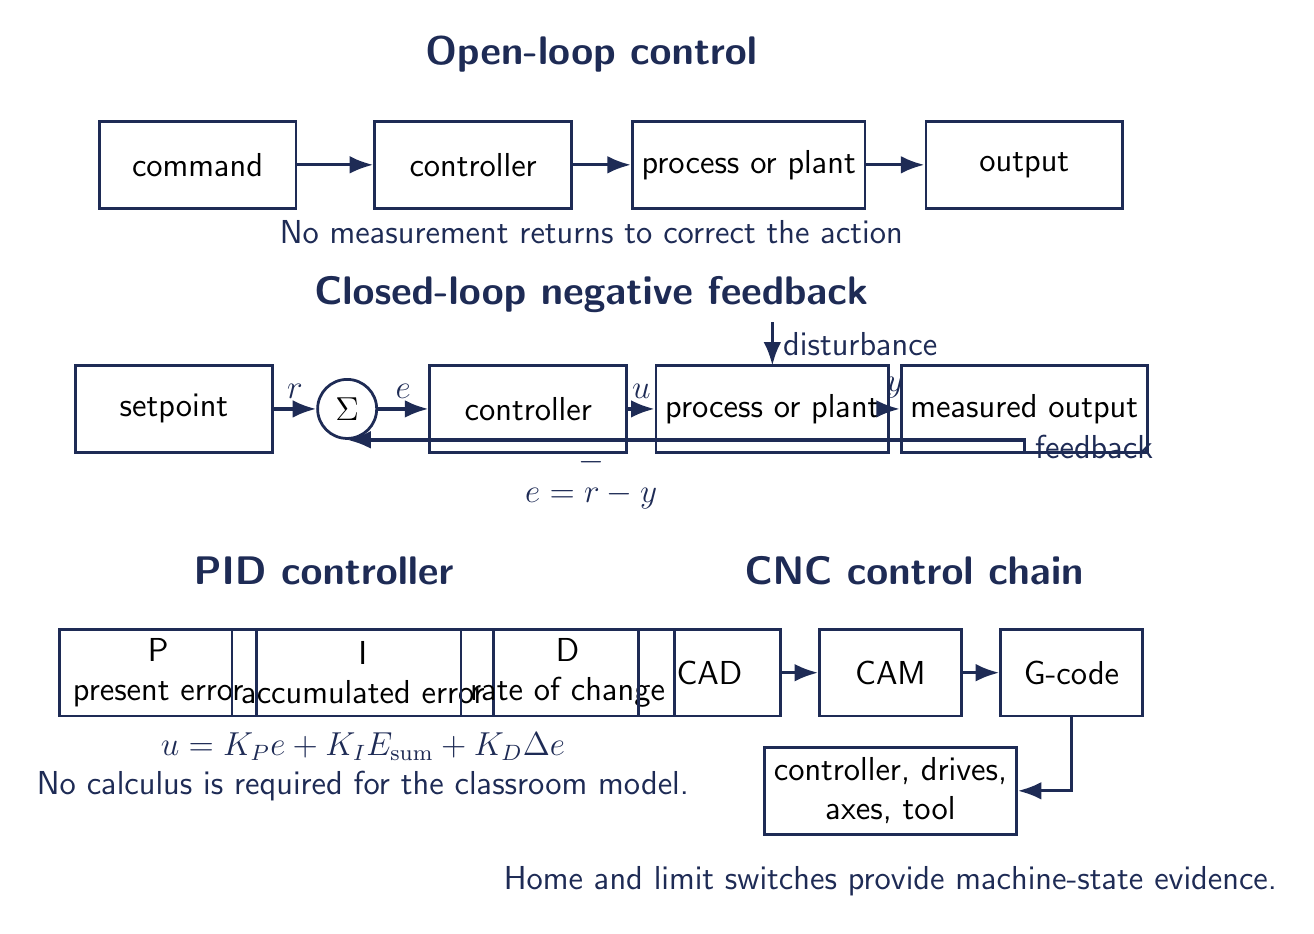
\begin{tikzpicture}[font=\large]
  \node[font=\bfseries\Large,text=TEJNavy] at (6.5,9.5) {Open-loop control};
  \node[block] (command) at (1.5,8.1) {command};
  \node[block] (controller) at (5.0,8.1) {controller};
  \node[block] (plant) at (8.5,8.1) {process or plant};
  \node[block] (output) at (12.0,8.1) {output};
  \draw[flow] (command) -- (controller);
  \draw[flow] (controller) -- (plant);
  \draw[flow] (plant) -- (output);
  \node[text=TEJNavy] at (6.5,7.25) {No measurement returns to correct the action};

  \node[font=\bfseries\Large,text=TEJNavy] at (6.5,6.45) {Closed-loop negative feedback};
  \node[block] (setpoint) at (1.2,5.0) {setpoint};
  \node[sum] (error) at (3.4,5.0) {$\Sigma$};
  \node[block] (control2) at (5.7,5.0) {controller};
  \node[block] (plant2) at (8.8,5.0) {process or plant};
  \node[block] (out2) at (12.0,5.0) {measured output};
  \draw[flow] (setpoint) -- node[above] {$r$} (error);
  \draw[flow] (error) -- node[above] {$e$} (control2);
  \draw[flow] (control2) -- node[above] {$u$} (plant2);
  \draw[flow] (plant2) -- node[above] {$y$} (out2);
  \draw[flow] (out2.south) |- node[pos=.25,right] {feedback} node[pos=.82,below] {$-$} (error.south);
  \draw[flow] (8.8,6.1) -- (8.8,5.55) node[midway,right] {disturbance};
  \node[text=TEJNavy] at (6.5,3.9) {$e=r-y$};

  \node[font=\bfseries\Large,text=TEJNavy] at (3.1,2.95) {PID controller};
  \node[block] (p) at (1.0,1.65) {P\\present error};
  \node[block] (i) at (3.6,1.65) {I\\accumulated error};
  \node[block] (d) at (6.2,1.65) {D\\rate of change};
  \node[text=TEJNavy,align=center] at (3.6,0.45) {$u=K_Pe+K_I E_{\mathrm{sum}}+K_D\Delta e$\\No calculus is required for the classroom model.};

  \node[font=\bfseries\Large,text=TEJNavy] at (10.6,2.95) {CNC control chain};
  \node[block,minimum width=1.8cm] (cad) at (8.0,1.65) {CAD};
  \node[block,minimum width=1.8cm] (cam) at (10.3,1.65) {CAM};
  \node[block,minimum width=1.8cm] (gcode) at (12.6,1.65) {G-code};
  \draw[flow] (cad) -- (cam);
  \draw[flow] (cam) -- (gcode);
  \node[block,minimum width=2.2cm] (machine) at (10.3,0.15) {controller, drives,\\axes, tool};
  \draw[flow] (gcode) |- (machine.east);
  \node[text=TEJNavy,align=center] at (10.3,-1.0) {Home and limit switches provide machine-state evidence.};
\end{tikzpicture}
\end{document}
